% Chapter Template

\chapter{Ensayos y Resultados} % Main chapter title

\label{Chapter4} % Change X to a consecutive number; for referencing this chapter elsewhere, use \ref{ChapterX}

%----------------------------------------------------------------------------------------
%	SECTION 1
%----------------------------------------------------------------------------------------
En este capitulo se presentan los ensayos realizados para validar el funcionamiento del equipo desarrollado.

\section{Ensayos de hardware}
\label{sec:pruebasHW}

A lo largo del desarrollo de este trabajo se implementaron diversas piezas de hardware. Algunas de ellas se trataban simplemente de etapas de adaptación de niveles de señales y otras más complejas como, los puertos del módulo principal, representaron un desafío y es por esto que merecen una mención detallada de los ensayos que fueron realizados sobre ellos. En particular el punto clave en este trabajo fue el hardware de la interfaz UART optoaislada de la que se ha hablado ampliamente es esta memoria y además fue sometida a prueba. Otro ensayo menos complejo, pero que aún así merece ser presentado en esta memoria es el ensayo de calibración de ADCs, ya que de ello depende el correcto funcionamiento de las pruebas de drivers.

\subsection{Ensayo de UART optoaislada}

Este ensayo buscó someter a un funcionamiento intensivo de la misma. Para ello se montó el banco de pruebas cuyo diagrama de conexión se presenta en la figura \ref{fig:BancoPruebaUart}. En este banco de pruebas se utiliza un adaptador USB-RS232 conectado a una computadora, cumpliendo la función de maestro en el protocolo establecido en la sección \ref{sec:UARTopto}, y los puertos del módulo principal cumplen la función de esclavos para la que fueron diseñados.

\begin{figure}[H]
	\centering
	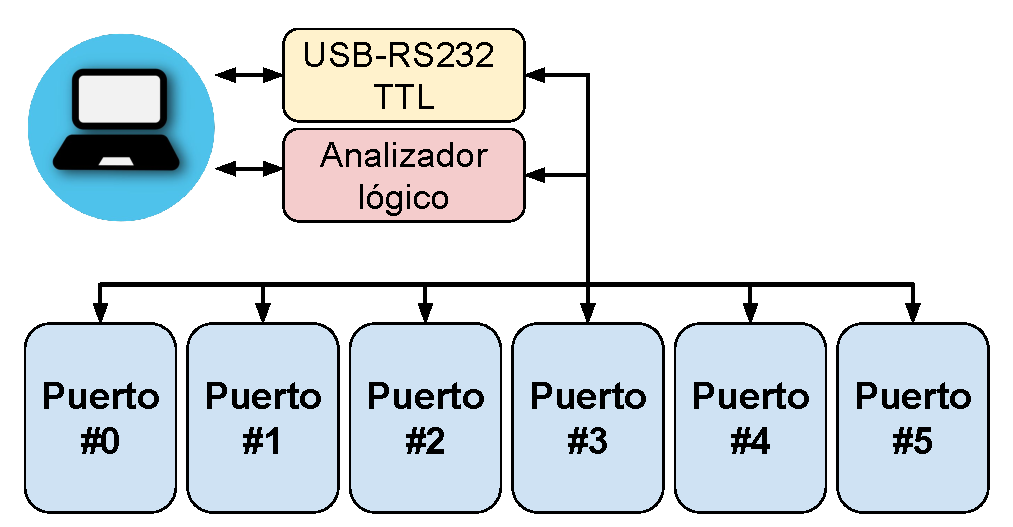
\includegraphics[width=0.6\textwidth]{./Figures/BancoPruebaUart.pdf}
	\caption{Diagrama del banco de pruebas de la interfaz UART optoaislada.}
	\label{fig:BancoPruebaUart}
\end{figure}

El ensayo de esta interfaz consiste en generar seis tramas de 5 bytes cada una acordes al protocolo, de modo que cada trama está dirigida a uno de los puertos y solo ese puerto responda a dicha trama. Este proceso se repitió 10.000 veces consecutivamente utilizando la terminal HTerm que permite hacer este tipo de automatización y se analizaron las respuestas de cada uno de los puertos. 
En la figura \ref{fig:AtaqueBytes} se puede ver una captura de la aplicación HTerm con el resultado del ensayo. Allí se puede ver en primera instancia que fueron enviados 300.000 bytes que corresponden a las seis tramas de 5 bytes enviadas 10.000 veces. En la imagen, además, está resaltado el número de bytes recibidos que totalizan 240.000, estos corresponden a los 4 bytes de la respuesta de cada uno de los 6 puertos.
Con este breve análisis se puede afirmar que durante la comunicación el volumen de datos fue el correcto, pero no se puede asegurar que las respuestas a cada trama enviada por el maestro la haya respondido el módulo adecuado.
Es por eso que debieron analizarse las respuestas recibidas. Por tratarse de 10.000 respuestas por cada módulo no es viable analizar una por una, entonces se optó por verificar la dirección del puerto correspondiente a cada respuesta, que se puede ver en el primer byte de cada una. Así se puede ver que las direcciones de las respuestas se repiten cada 24 bytes y afirmar que los puertos responden únicamente a las tramas que le corresponden.

\begin{figure}[H]
	\centering
	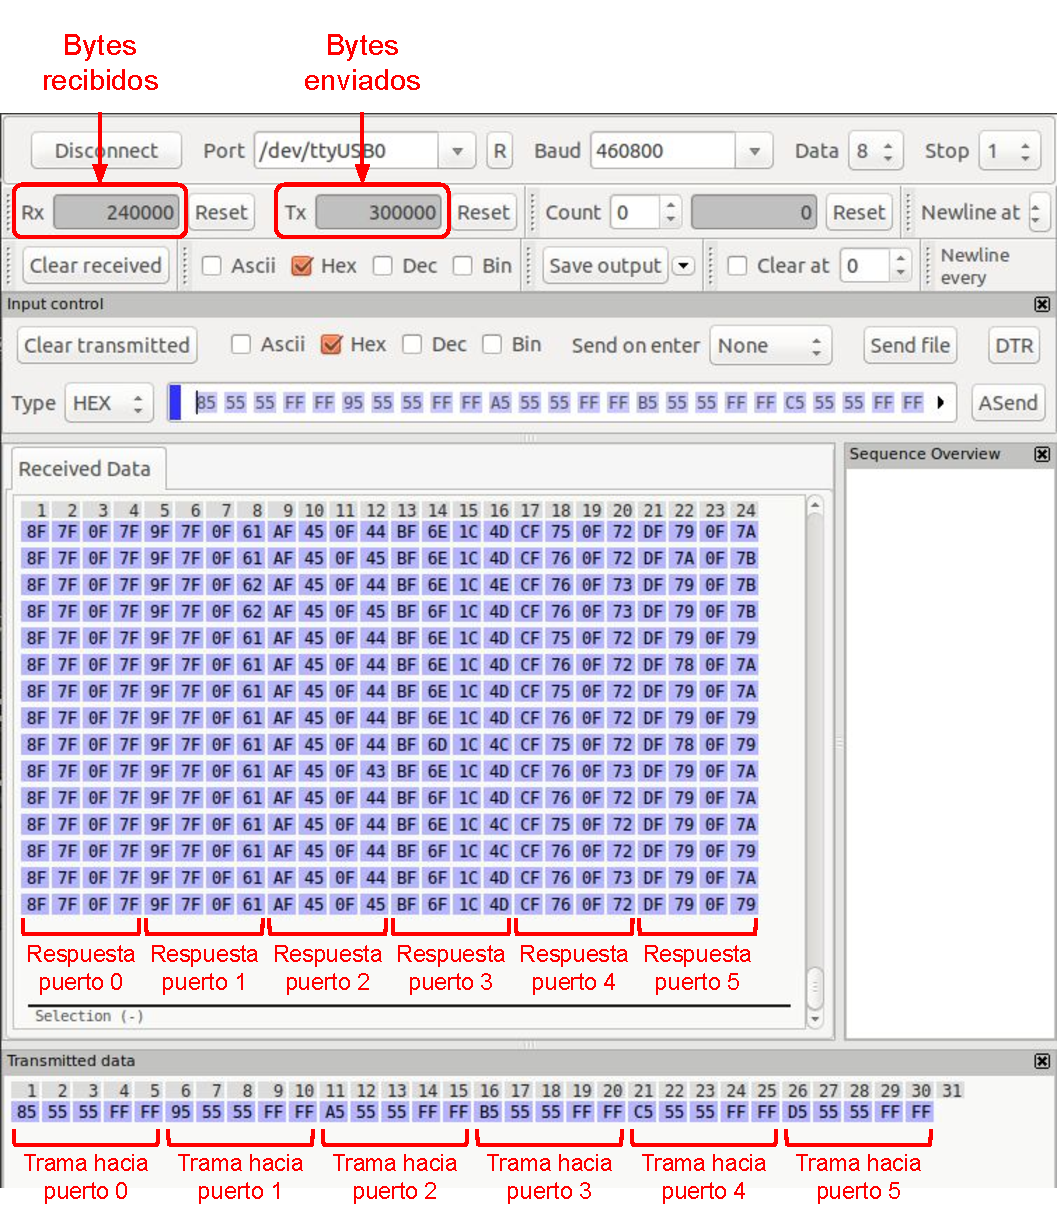
\includegraphics[width=0.85\textwidth]{./Figures/AtaqueBytes.pdf}
	\caption{Captura de la terminal serie al concluir el envío de tramas.}
	\label{fig:AtaqueBytes}
\end{figure}

En la figura \ref{fig:BancoPruebaUart} también se puede ver la conexión de un analizador lógico. Esto se debe a que una parte del ensayo consiste en corroborar el correcto desempeño del protocolo. 
Un punto importante del protocolo es el agregado a la trama que envía el maestro de dos bytes que no transportan información. Estos bytes extra fueron incluidos con el único fin de evitar la superposición entre las respuestas de los puertos. 
La figura \ref{fig:CapturaAnalizador} es una captura, realizada con un analizador, de una trama enviada y su respuesta. Allí se puede apreciar que gracias al agregado de dos bytes vacíos se logra tener un espacio libre antes de que otro módulo pueda responder.

\begin{figure}[H]
	\centering
	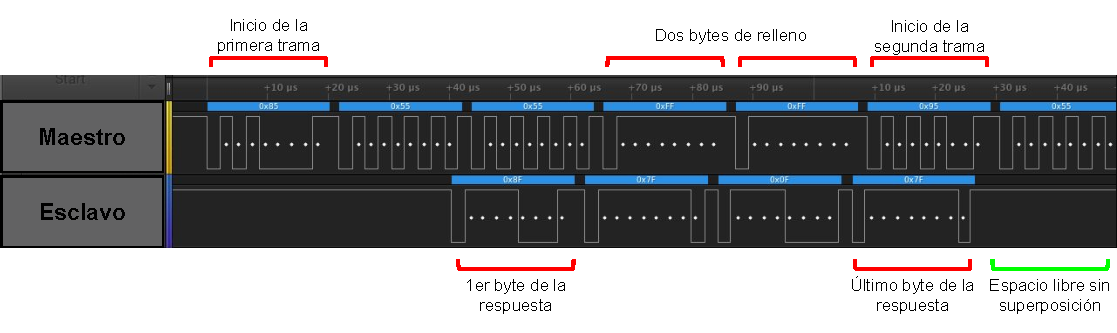
\includegraphics[width=1\textwidth]{./Figures/CapturaAnalizador.pdf}
	\caption{Captura de la comunicación maestro-esclavo.}
	\label{fig:CapturaAnalizador}
\end{figure}

\subsection{Calibración de ADCs}

Si bien este trabajo no consiste en el desarrollo de un instrumento de medición y no se establecieron requerimientos de precisión, es una buena práctica caracterizar las mediciones que realiza el equipo y si es posible hacer correcciones. 
Los ADCs del módulo principal son los principales encargados de las mediciones analogicas que realiza el equipo. Por ello se decidió realizar una contrastación de las mediciones de estos conversores con un instrumento patrón. Para hacer este ensayo se montó el banco de pruebas de la figura \ref{fig:BancoCal}

\begin{figure}[H]
	\centering
	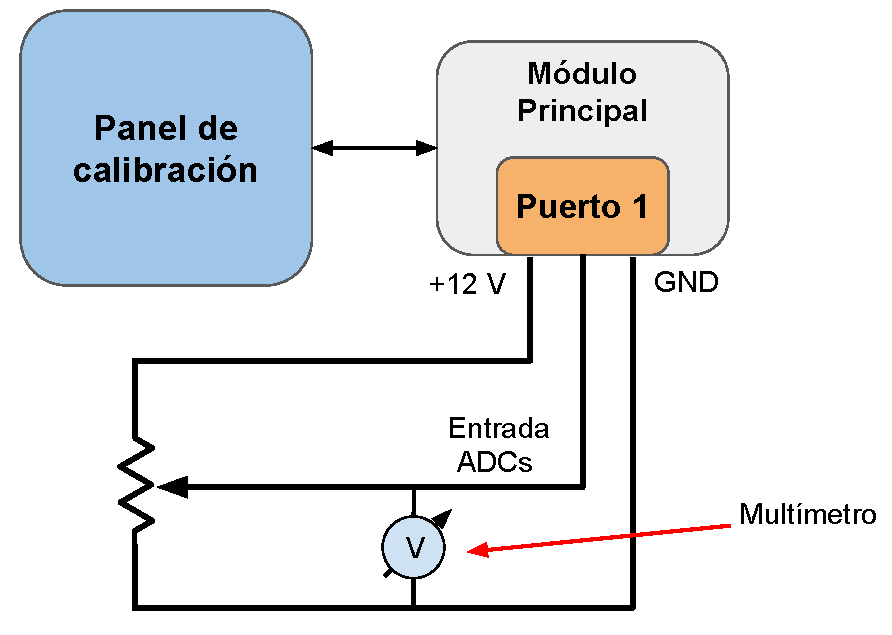
\includegraphics[width=0.75\textwidth]{./Figures/BancoCal.pdf}
	\caption{Banco de pruebas para la calibración de ADCs.}
	\label{fig:BancoCal}
\end{figure}

El ensayo consiste en establecer la misma tensión de entrada a los dos canales analógicos de cada puerto y comparar la medición indicada por el multímetro con la indicación en la interfaz de usuario. El multimetro que se utilizó para la contrastación es un multímetro Fluke 107 con su calibracion de fabrica del año 2016.
En la figura \ref{fig:CalADCs} corresponde a la calibración del canal analogico 0 de los 6 puertos. En primera instancia se parece mucho al comportamiento lineal esperado, pero si se presta atencion al grafico de la figura \ref{fig:CalADCzoom} podemos ver la zona de mediciones más cercanas al cero ampliada. En este gráfico se aprecia mejor la diferencia que hay entre las mediciones de los ADCs y la recta ideal de medición. Esta diferencia se mantiene casi constante en todo el rango. Otra cosa que se puede ver en el gráfico es que para tensiones por debajo de los 200 mV  la curva se torna no lineal.
Estas dos diferencias con la curva ideal tienen una misma causa y es un error de Offset en la medición posiblemente producido por una diferencia de potencial entre la masa del ADC y la del amplificador de entrada. 

\begin{figure}[H]
	\centering
	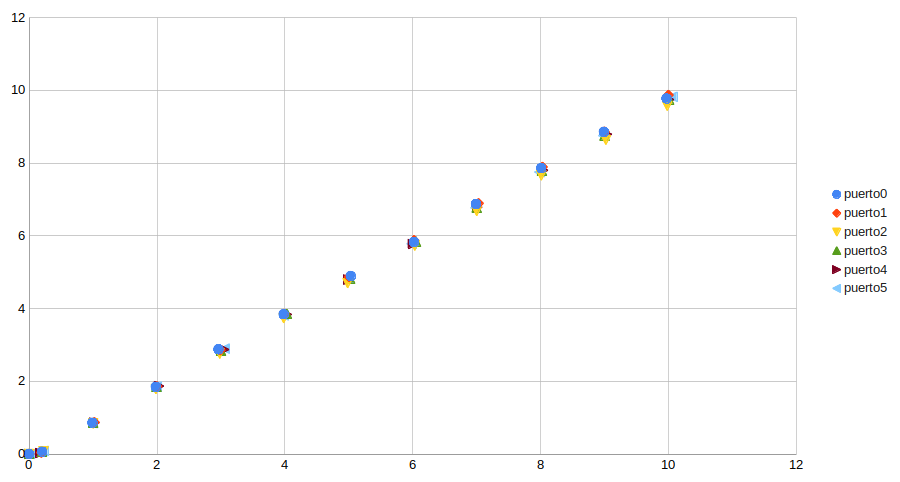
\includegraphics[width=1\textwidth]{./Figures/CalADCs.png}
	\caption{Calibración de ADCs.}
	\label{fig:CalADCs}
\end{figure}

\begin{figure}[H]
	\centering
	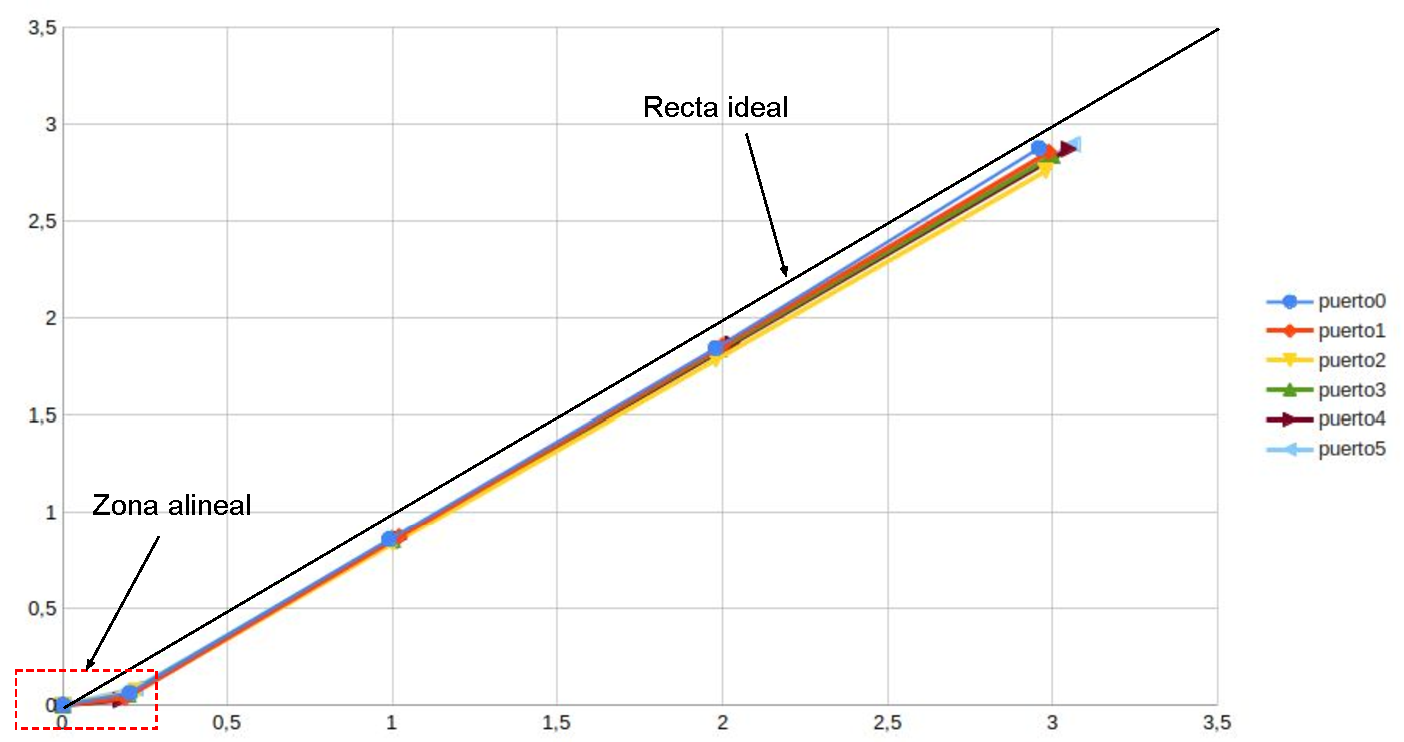
\includegraphics[width=1\textwidth]{./Figures/CalADCzoom.pdf}
	\caption{Calibración de ADCs, zoom cerca del cero.}
	\label{fig:CalADCzoom}
\end{figure}

Para mitigar los efectos del offset, se hizo una corrección por software. 
Luego se repitió el ensayo obteniendo el gráfico de la figura \ref{fig:CorregidoCalADCzoom}. En este nuevo ensayo se ve que la diferencia entre la medición de los ADCs y la recta ideal se redujo, pero la alinealidad en la parte baja persiste y solo podría corregirse por hardware. Sin embargo esto no representa un problema ya que todas las mediciones que se realizan en las pruebas están por encima de los 200 mV.

\begin{figure}[H]
	\centering
	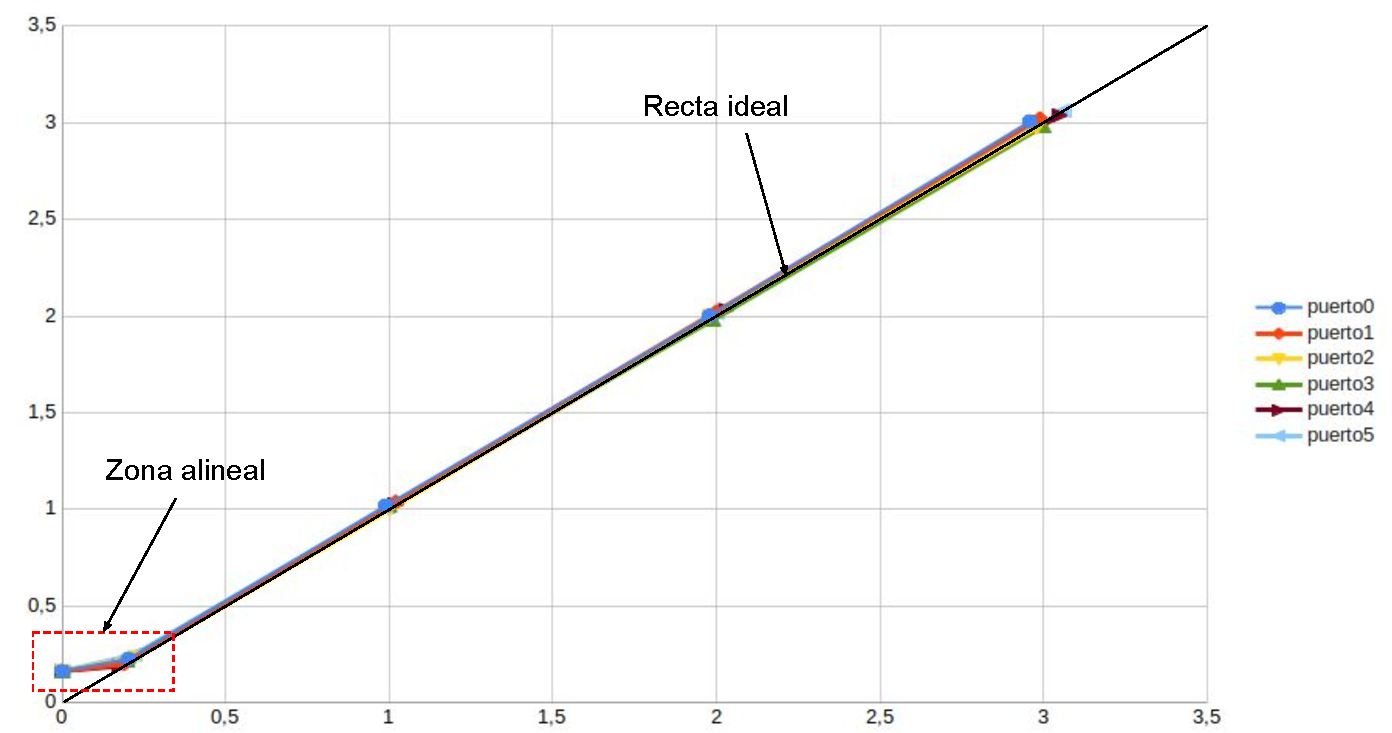
\includegraphics[width=1\textwidth]{./Figures/CorregidoCalADCzoom.pdf}
	\caption{Calibración de ADCs luego de corrección de offset por software}
	\label{fig:CorregidoCalADCzoom}
\end{figure}


\section{Pruebas de integración}

Las pruebas de integración buscar ensayar al equipo en forma integral. De este modo se prueba el correcto comportamiento e interacción entre las partes que componen al sistema en distintas  condiciones de uso posibles. 
Una forma de hacer este tipo de pruebas es mediante la ejecución de casos de uso.
Dos casos de uso muy importantes son el de la prueba de temporizadores y el de prueba de driver. Las tablas \ref{tab:CasoDriver} y \ref{tab:CasoTemp} indican paso a paso la secuencia de ambos casos de uso.
En el caso de la prueba de temporizadores como precondición se requiere que el temporizador esté conectado al banco de pruebas. Para el ensayo se escogió un temporizador marca Secuen, modelo TGE de cuatro terminales.
Por otro lado, en el caso de la prueba de drivers se utilizó un driver marca Meanwell, modelo ELG-150-C700B conectado a una carga LED de 70 W a 700 mA.
Los dos casos de uso se pusieron a prueba y verificaron cada uno de los pasos satisfactoriamente.




% Please add the following required packages to your document preamble:
% \usepackage{multirow}
% \usepackage{graphicx}
\begin{table}[ht]
\centering
\caption[Caso de uso de prueba de drivers]{Caso de uso de prueba de drivers}
\resizebox{\textwidth}{!}{%
\begin{tabular}{lllc}
\hline
\multicolumn{2}{l}{\textbf{Título}}                     & \textbf{Descripción}                                                                                                                        & \multicolumn{1}{l}{\textbf{Verifica}} \\ \hline
\multicolumn{2}{l}{Nombre}                              & Prueba de Drivers                                                                                                                           & \multicolumn{1}{l}{}                  \\ \hline
\multirow{3}{*}{}  & Breve descripción                  & \begin{tabular}[c]{@{}l@{}}Ejecución de la prueba de drivers para \\ luminarias LED \end{tabular}                                            & \multicolumn{1}{l}{}                  \\
                   & Actor principal                    & Operario                                                                                                                                    & \multicolumn{1}{l}{}                  \\
                   & Disparadores                       & Presionar en pantalla el botón de Marcha                                                                                                    & \multicolumn{1}{l}{}                  \\ \hline
\multicolumn{2}{l}{Flujo de eventos}                    &                                                                                                                                             & \multicolumn{1}{l}{}                  \\ \hline
\multirow{13}{*}{} & \multirow{9}{*}{Flujo Básico}      & 1. Se presiona en pantalla el botón de Marcha.                                                                                              & \multicolumn{1}{l}{}                  \\
                   &                                    & \begin{tabular}[c]{@{}l@{}}2. El banco de pruebas alimenta el driver y se \\ dimeriza al 10\%\end{tabular}                                  & SI                                    \\
                   &                                    & \begin{tabular}[c]{@{}l@{}}3. Se miden los valores de tensión y corriente \\ del driver \end{tabular}                                        & SI                                    \\
                   &                                    & \begin{tabular}[c]{@{}l@{}}4. Si las mediciones están dentro de los valores \\ de aceptación, se dimeriza al 50\%\end{tabular}              & SI                                    \\
                   &                                    & \begin{tabular}[c]{@{}l@{}}5. Se miden los valores de tensión y corriente \\ del driver\end{tabular}                                        & SI                                    \\
                   &                                    & \begin{tabular}[c]{@{}l@{}}6. Si las mediciones están dentro de los valores \\ de aceptación, se dimeriza al 100\%\end{tabular}             & SI                                    \\
                   &                                    & \begin{tabular}[c]{@{}l@{}}7. Se miden los valores de tensión y corriente \\ del driver\end{tabular}                                        & SI                                    \\
                   &                                    & \begin{tabular}[c]{@{}l@{}}8. Si las mediciones están dentro de los valores de\\ aceptación, se indica en pantalla PASA\end{tabular}        & SI                                    \\
                   &                                    & 9. Esperar nueva prueba.                                                                                                                    & SI                                    \\ \cline{2-4} 
                   & \multirow{4}{*}{Flujo Alternativo} & Del punto 3, 5 o 7 del flujo básico                                                                                                         & \multicolumn{1}{l}{}                  \\
                   &                                    & \begin{tabular}[c]{@{}l@{}}4A. Si las mediciones no están dentro de los valores \\ de aceptación se aborta la prueba.\end{tabular}          & SI                                    \\
                   &                                    & 5A. Se indica en pantalla NO PASA                                                                                                           & SI                                    \\
                   &                                    & Se regresa al punto 9 del flujo básico                                                                                                      & SI                                    \\ \hline
\multicolumn{2}{l}{Requerimientos especiales}           &                                                                                                                                             & \multicolumn{1}{l}{}                  \\ \hline
\multicolumn{2}{l}{Precondiciones}                      & El driver debe estar conectado al banco de pruebas.                                                                                         & SI                                    \\ \hline
\multicolumn{2}{l}{Poscondiciones}                      & \begin{tabular}[c]{@{}l@{}}Se debe desconectar la alimentación del driver \\ (por software) para poder operar en forma segura.\end{tabular} & SI                                    \\ \hline
\end{tabular}%
}
\label{tab:CasoDriver}
\end{table}



% Please add the following required packages to your document preamble:
% \usepackage{multirow}
% \usepackage{graphicx}
\begin{table}[ht]
\centering
\caption[Caso de uso de prueba de temporizadores]{Caso de uso de prueba de temporizadores}
\resizebox{\textwidth}{!}{%
\begin{tabular}{lllc}
\hline
\multicolumn{2}{l}{\textbf{Título}}                                                               & \textbf{Descripción}                                                                                                                                                                             & \textbf{Verifica}    \\ \hline
\multicolumn{2}{l}{Nombre}                                                                        & Prueba de Temporizadores                                                                                                                                                                         & \multicolumn{1}{l}{} \\ \hline
\multirow{3}{*}{}                       & Breve descripción                                       & Ejecución de la prueba de temporizadores                                                                                                                                                         & \multicolumn{1}{l}{} \\
                                        & Actor principal                                         & Operario                                                                                                                                                                                         & \multicolumn{1}{l}{} \\
                                        & Disparadores                                            & Presionar en pantalla el botón de Marcha                                                                                                                                                         & \multicolumn{1}{l}{} \\ \hline
\multicolumn{2}{l}{\textbf{Flujo de eventos}}                                                     &                                                                                                                                                                                                  & \multicolumn{1}{l}{} \\ \hline
\multirow{15}{*}{}                      & \multirow{11}{*}{Flujo Básico}                          & 1. Se presiona el botón (en pantalla) de Marcha                                                                                                                                                  & \multicolumn{1}{l}{} \\
                                        &                                                         & \begin{tabular}[c]{@{}l@{}}2. Ajustar el temporizador al tiempo T1 (minimo) \\ cuando se indique en pantalla.\end{tabular}                                                                       & SI                   \\
                                        &                                                         & \begin{tabular}[c]{@{}l@{}}3. El banco de pruebas activa el temporizador o\\  solicita presionar el pulsador.\end{tabular}                                                                       & SI                   \\
                                        &                                                         & 4. El temporizador activa su salida.                                                                                                                                                             & SI                   \\
                                        &                                                         & 5. Inicia la cuenta de tiempo de encendido.                                                                                                                                                      & SI                   \\
                                        &                                                         & \begin{tabular}[c]{@{}l@{}}6. Cuando finaliza el tiempo del temporizador, \\ si el tiempo esta dentro del rango definido se indica \\ ajustar el temporizador al tiempo T2 (maximo)\end{tabular} & SI                   \\
                                        &                                                         & \begin{tabular}[c]{@{}l@{}}7. El banco de pruebas activa el temporizador o \\ solicita presionar el pulsador.\end{tabular}                                                                       & SI                   \\
                                        &                                                         & 8. Inicia la cuenta de tiempo de encendido.                                                                                                                                                      & SI                   \\
                                        &                                                         & \begin{tabular}[c]{@{}l@{}}9. Cuando finaliza el tiempo del temporizador, si \\ el tiempo esta dentro del rango definido se detiene \\ la prueba.\end{tabular}                                   & SI                   \\
                                        &                                                         & 10. Se indica en pantalla PASA.                                                                                                                                                                  & SI                   \\
                                        &                                                         & 11. Esperar nueva prueba.                                                                                                                                                                        & SI                   \\ \cline{2-4} 
                                        & \multirow{4}{*}{Flujo Alternativo}                      & Del punto 5 o del punto 8 del flujo básico                                                                                                                                                       & \multicolumn{1}{l}{} \\
                                        &                                                         & \begin{tabular}[c]{@{}l@{}}6A. Cuando finaliza el tiempo del temporizador, \\ si el tiempo encendido no está dentro de los \\ valores aceptables se aborta la prueba.\end{tabular}               & SI                   \\
                                        &                                                         & 7A. Se indica indica en pantalla NO PASA                                                                                                                                                         & SI                   \\
                                        &                                                         & Se regresa al punto 11 del flujo básico                                                                                                                                                          & SI                   \\ \hline
\multicolumn{2}{l}{\textbf{\begin{tabular}[c]{@{}l@{}}Requerimientos \\ especiales\end{tabular}}} & -                                                                                                                                                                                                & \multicolumn{1}{l}{} \\ \hline
\multicolumn{2}{l}{\textbf{Precondiciones}}                                                       & \begin{tabular}[c]{@{}l@{}}El temporizador debe estar conectado al banco \\ de pruebas.\end{tabular}                                                                                             & SI                   \\ \hline
\multicolumn{2}{l}{\textbf{Poscondiciones}}                                                       & \begin{tabular}[c]{@{}l@{}}Se debe desconectar la alimentación del \\ temporizador (por software) para poder \\ operar en forma segura.\end{tabular}                                             & SI                   \\ \hline
\end{tabular}%
}
\label{tab:CasoTemp}
\end{table}
